\documentclass[11pt,aspectratio=169]{beamer}
\usetheme{Madrid}
 
% ---------- Micro-typography ----------
\usepackage[expansion=false]{microtype}
 
% ---------- Math & symbols ----------
\usepackage{mathtools}          % includes amsmath
\usepackage{amssymb,amsfonts}
 
% ---------- Graphics / colors / tables ----------
\usepackage{graphicx}
\usepackage[table]{xcolor}      % includes colortbl
\usepackage{float}              % [H] placement for figures
\usepackage{booktabs}

 
% ---------- Bibliography ----------
\usepackage{natbib}
 
% ---------- Misc ----------
\usepackage{etoolbox}
\pdfstringdefDisableCommands{\def\translate#1{#1}}
 
 
% ==================================================
%                 COLOR PALETTE
% ==================================================
 
\definecolor{darkpink}{RGB}{139,0,75}
\definecolor{lightsoftpink}{RGB}{250,225,235}
 
 
% ==================================================
%              BEAMER LOOK-AND-FEEL
% ==================================================
 
% Frame titles
\setbeamercolor{frametitle}{fg=white,bg=darkpink}
\setbeamertemplate{frametitle}{%
  \nointerlineskip%
  \begin{beamercolorbox}[wd=\paperwidth,ht=3ex,dp=1.5ex,leftskip=0.7cm]{frametitle}
    \insertframetitle
  \end{beamercolorbox}%
}
 
% Structure color (bullets, numbering, etc.)
\setbeamercolor{structure}{fg=darkpink}
 
% Background
\setbeamercolor{background canvas}{bg=white}
 
% Blocks
\setbeamercolor{block title}{bg=darkpink,fg=white}
\setbeamercolor{block body}{bg=lightsoftpink,fg=black}
 
% Remove footline
\setbeamertemplate{footline}{}
\addtobeamertemplate{title page}{\vspace*{-0.5\baselineskip}}{}
 
 
% ==================================================
%               CONVENIENCE
% ==================================================
 
\setbeamertemplate{itemize items}[circle]
\setbeamertemplate{itemize subitem}{\tiny\raise1.5pt\hbox{\donotcoloroutermaths$\color{darkpink}\blacktriangleright$}}
\setbeamertemplate{itemize subsubitem}{\scriptsize\raise1.5pt\hbox{\donotcoloroutermaths$\color{darkpink}\bullet$}}
 
% ---------- Figure source note ----------
\newcommand{\source}[1]{\vspace{-0.5em}\par\footnotesize\textit{Source:} #1}
 
% Margins
\setbeamersize{text margin left=2em, text margin right=2em}
\addtolength{\leftmargini}{2em}
 
 
%%%%%%%%%%% ------ TITLE PAGE --------- %%%%%%%%%%%%%%%%%%%
\title{Does Female Leadership Relate to Productivity-Wage Gaps in Colombia? \\
{\small Applied Econometrics ECON 6375 Paper}}
\author{Ingri Katherine Quevedo Rocha}
\institute{\small \url{ingriq@gwu.edu} \\ George Washington University \\ M.S.\ Applied Economics (Spring 2026)}
\date{\today}
 
 
%%%%%%%%%%%%%%%%%%%%%%%%%%% BEGIN %%%%%%%%%%%%%%%%%%%%%%%
\begin{document}
 
\begin{frame}
  \titlepage
\end{frame}

%%%%%%----------------------%%%%%%
\begin{frame}{Introduction}
\begin{itemize}
  \item Across the world, workers are paid substantially less than the value they produce. For example, estimates for Colombia suggest workers produce approximately 40\% more than they earn.
  \item Microeconomic theory explains that the productivity-wage gap arises under imperfect competition where firms have wage-setting power.
  \item Yet this gap is not uniform: management structure shapes how aggressively firms exploit their wage-setting power.
  \item In particular, female leaders place greater weight on worker welfare and are less likely to engage in anticompetitive behavior.
\end{itemize}
\vspace{0.5em}
\textbf{This paper examines whether firms with a larger share of female leaders are associated with a lower productivity-wage gap.}
\end{frame}

%%%%%%----------------------%%%%%%
\begin{frame}{Data}

\begin{itemize}
  \item Firm-level data from the Annual Manufacturing Survey (Encuesta Anual Manufacturera, EAM) of Colombia.
  \item Unbalanced panel of 11,235 firms between 2000-2019.
  \item Manufacturing sectors in developing economies are dominated by small and medium-sized enterprises.
\end{itemize}

\begin{table}
\centering
\footnotesize
\caption{Descriptive Statistics}
\label{tab:desc_stats}
\begin{tabular}{lrrrrrr}
\toprule
Variable & Mean & SD & Min & Median & Max \\
\midrule
Share of female executives (\%) & 45.192 & 39.925 & 0.000 & 49.812 & 100.000 \\
Firm's share of industry employment (\%) & 0.020 & 0.066 & 0.000 & 0.004 & 1.000 \\
Share of workers in production (\%) & 61.951 & 21.743 & 0.000 & 66.667 & 100.000 \\
Gross output (\$ millions USD) & 1.219 & 536.010 & 756.959 & 11.356 & 2,968.214 \\
Firm age (years) & 4.262 & 3.422 & 1 & 3 & 20 \\
Number of workers & 56 & 146 & 1 & 20 & 4921 \\
Wage per worker (\$ thousands USD) & 1.827 & 91 & 349.180 & 2.296 & 1,498.014 \\
\bottomrule
\end{tabular}
\end{table}

\end{frame}
%%%%%%----------------------%%%%%%

\begin{frame}{Productivity-Wage Gap Definition}

Following Yeh et al. (2022) we obtain the firm's markdown ($\nu$) as:

\begin{equation}
\nu \equiv \frac{R'(L)}{w(L)} = \varepsilon_L^{-1}+1
\end{equation}

After some algebraic manipulation using the production approach by De Locker et al. (2020):

\begin{equation}
    \nu = \frac{\theta^L}{\theta^M} \cdot 
    \frac{{p^m} M}{w(L)L}.
\end{equation}

Where $\theta^L$ and $\theta^M$ are the input-output elasticities of labor and materials.

\end{frame}

%%%%%%----------------------%%%%%%

\begin{frame}{Markdown estimation - Production Approach}

Translog production function GMM estimation:

\begin{flalign}
\begin{aligned}
\log(\mathit{GO}_{it}) &= \beta_{0} + \beta_{1}\log(K_{it}) + \beta_{2}\log(L_{it}) + \beta_{3}\log(M_{it}) + \beta_{4}(\log K_{it})^2 + \beta_{5}(\log L_{it})^2 \\
& + \beta_{6}(\log M_{it})^2 + \beta_{7}\log(K_{it})\log(L_{it}) + \beta_{8}\log(K_{it})\log(M_{it}) + \beta_{9}\log(L_{it})\log(M_{it}) \\
& + \gamma_t + \varepsilon_{it}.
\end{aligned}
\end{flalign}

As follows:
\vspace{-0.5em}
\begin{equation}
\begin{aligned}
    \hat{\theta}_{L,it} &= \hat{\beta}_{2} + 2\hat{\beta}_{5}\log(L_{it}) + \hat{\beta}_{7}\log(K_{it}) + \hat{\beta}_{9}\log(M_{it}), \\
    \hat{\theta}_{M,it} &= \hat{\beta}_{3} + 2\hat{\beta}_{6}\log(M_{it}) + \hat{\beta}_{8}\log(K_{it}) + \hat{\beta}_{9}\log(L_{it}).
\end{aligned}
\end{equation}

\end{frame}

%%%%%%----------------------%%%%%%
\begin{frame}{Markdown and Female Leadership}
\vspace{-0.5em}
\begin{figure}
    \centering
    \caption{Markdown and Female Leadership}
    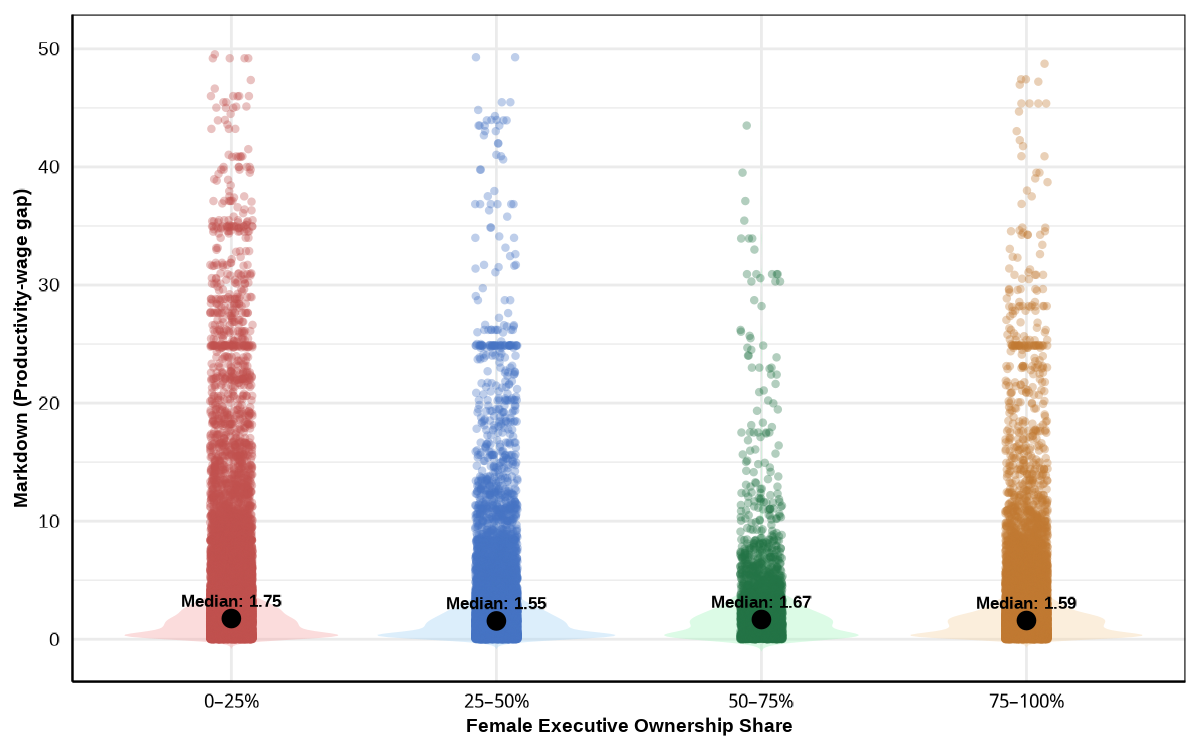
\includegraphics[width=\textwidth, height=0.7\textheight, keepaspectratio]{violin_markdown_ownwshare.png}
\end{figure}
\end{frame}


%%%%%%----------------------%%%%%%
\begin{frame}{Empirical Framework}

Linear regression model:

\begin{align}
  \log(\text{Markdown}_{it}) = \alpha + \beta \, \text{FemaleLeadership}_{it} + \boldsymbol{\gamma}' \mathbf{X}_{it} + \alpha_t + \alpha_s + \alpha_r + \varepsilon_{it}
\end{align}

where:
\begin{itemize}
  \item $\log(\text{Markdown}_{it})$ is the logarithm of the productivity-wage gap for firm $i$ in year $t$
  \item $\text{FemaleLeadership}_{it}$ denotes the share of women in executive and ownership positions
  \item The vector $\mathbf{X}_{it}$ includes a rich set of firm-level controls designed to isolate the leadership channel from confounding variation in productivity, scale, and workforce composition.
  \item $\alpha_t$, $\alpha_s$, and $\alpha_r$ are year, industry, and region fixed effects.
  \item $\varepsilon_{it}$ is the error term.
\end{itemize}

\end{frame}

%%%%%%----------------------%%%%%%
\begin{frame}{Regression Results}
\vspace{-0.8em}
\begin{table}
\centering
\footnotesize
\caption{Regression Results - Dependent variable: log(Markdown)}
\begin{tabular}{lcccc}
\hline
 & (1) & (2) & (3) \\
\hline
Share of Female Executives & -0.0010*** & -0.0010*** & -0.0011*** \\
 & (0.0001) & (0.0002) & (0.0002) \\
Firm's share of employment in the industry &  & 2.0356*** & 2.4268*** \\
 &  & (0.3723) & (0.3713) \\
Share of production workers &  & -0.0021*** & -0.0018*** \\
 &  & (0.0003) & (0.0003) \\
Industry HHI &  & 0.5729*** & 0.5719*** \\
 &  & (0.0634) & (0.0635) \\
TFP &  & 0.1557*** & 0.1578*** \\
 &  & (0.0039) & (0.0039)\\
\hline
Additional controls &  & Size \& Age & Size \& Age\\
FE: Year & X & X & X\\
FE: Region & X &  & X \\
FE: Industry & X &  &  \\
\hline
$N$ & 48,292 & 31,664 & 31,664 \\
$R^{2}$ & 0.5097 & 0.1243 & 0.1386 \\
\hline
\multicolumn{4}{l}{\textit{Note:} $^{***}p<0.001$; $^{**}p<0.01$; $^{*}p<0.05$; $^{.}p<0.1$} \\
\end{tabular}
\end{table}

\end{frame}

%%%%%%----------------------%%%%%%
\begin{frame}{Conclusion}
\begin{itemize}
  \item Management structure is a meaningful margin of variation in firms' wage-setting behavior.
  \item A larger share of female executives is associated with less aggressive exploitation of monopsony rents.
  \item This is consistent with evidence that female leaders place greater weight on worker welfare and interpret productivity signals differently from their male counterparts.
  \item Policies promoting gender diversity in executive and ownership positions (board gender quotas, bias-free promotion practices, and mentorship pipelines) can increase worker welfare, reduce monopsony power and increase overall economic efficiency.
\end{itemize}
\end{frame}

\end{document}